\documentclass{article} % Defines the document class, article is commonly used
\usepackage[shortlabels]{enumitem}
\usepackage{amsmath}    % Allows for more advanced math formatting
\usepackage{amssymb}    % Provides additional mathematical symbols
\usepackage{amsthm}     % \qed
\usepackage{graphicx}   % image
\usepackage{float}      % image placement
\usepackage{hyperref}
\hypersetup{
    colorlinks=true,       % false: boxed links; true: colored links
    linkcolor=black,       % color of internal links
}
\usepackage[margin=1.5in]{geometry}
\usepackage{siunitx}

\begin{document}

\title{EEC133 HW3}
\author{Tao Wang}
\date{\today}

\maketitle
\tableofcontents

\section{A few simple dipole antennas}
\begin{enumerate}[(a)]
      \item
            \[f = 100 \times 10^6 \text{ Hz, } \lambda = \frac{c}{f} = 3 \text{ m, } l = 5 \times 10^{-2} \text{ m, } I_0 = 0.5 \text{ A }\]
            \begin{enumerate}[(i)]
                  \item $\boxed{\text{Yes}}$, the antenna could be model as a Hertzian Dipole because $50 < \frac{\lambda}{l} = 60$
                  \item For a Hertzian Dipole,
                        \[S_{max} = \frac{\eta_0 k^2 I_0 ^2 l^2}{32 \pi^2 R^2} \approx \frac{15 \pi I_0 ^2}{R^2}\left(\frac{l}{\lambda}\right)^2\]

                        Here, R = 1 mile = $1.6 \times 10^3 \text{ m}$

                        Plug in all values:

                        \[\boxed{S_{max} = 1.28 \si{\frac{nW}{m^2}}}\]
                  \item
                        For a Hertzian Dipole

                        \[|\widetilde{E}| = \frac{I k l \eta_0}{4 \pi R}\]

                        Therefore,

                        \[|\widetilde{E}|_{rms} = \frac{I_0 k l \eta_0}{4 \pi R \sqrt{2}}\]
                        \[= \boxed{0.69 \si{\frac{mV}{m}}}\]
                  \item
                        Since the antenna is a Hertzian Dipole, $F(\theta, \phi) = \sin^2(\theta)$.

                        Next,we have the total radiated power in all direction as
                        \[P_{rad} = R^2 S_{max}\int_{\text{ sphere }}  F(\theta, \phi) d\Omega\]

                        For Hertzian Dipole, $P_{rad} = \frac{8 \pi}{3}$.

                        To get the total power radiated between $\theta = 85^{\circ} \text{ and } 95^{\circ}$, change the integration bounds.

                        \[P_{85-95} = R^2 S_{max}\int_{0}^{2\pi} \int_{85^{\circ}}^{95^{\circ}}  F(\theta, \phi) d\Omega\]

                        Therefore,
                        \[\frac{P_{85-95}}{P_{rad}} = \frac{\int_{0}^{2\pi} \int_{85^{\circ}}^{95^{\circ}}  F(\theta, \phi) d\Omega}{\int_{\text{ sphere }}  F(\theta, \phi) d\Omega} = 0.13 = \boxed{13 \%}\]
            \end{enumerate}
      \item
            \[f = 100 \times 10^6 \text{ Hz, } \lambda = \frac{c}{f} = 3 \text{ m, } l = 10 \times 10^{-2} \text{ m, } I_0 = 0.5 \text{ A }\]
            \begin{enumerate}[(i)]
                  \item $\boxed{\text{No}}$, the antenna could not be model as a Hertzian Dipole because $50 < \frac{\lambda}{l} = 30$. However, it could be modeled as a \textit{Small Dipole Antenna} because $10 < 30$
                  \item For a Small Dipole,
                        \[S_{max} = \frac{\eta_0 k^2 I_0 ^2 l^2}{(4)32 \pi^2 R^2} \approx \frac{15 \pi I_0 ^2}{4R^2}\left(\frac{l}{\lambda}\right)^2\]

                        Here, R = 1 mile = $1.6 \times 10^3 \text{ m}$

                        Plug in all values:

                        \[\boxed{S_{max} = 1.28 \si{\frac{nW}{m^2}}}\]
                  \item
                        For a Small Dipole

                        \[|\widetilde{E}| = \frac{I k l \eta_0}{(2)4 \pi R}\]

                        Therefore,

                        \[|\widetilde{E}|_{rms} = \frac{I_0 k l \eta_0}{(2)4 \pi R \sqrt{2}}\]
                        \[= \boxed{0.69 \si{\frac{mV}{m}}}\]
                  \item
                        Since the antenna is a Small Dipole, $F(\theta, \phi) = \sin^2(\theta)$.

                        Next,we have the total radiated power in all direction as
                        \[P_{rad} = R^2 S_{max}\int_{\text{ sphere }}  F(\theta, \phi) d\Omega\]

                        For Small Dipole, $P_{rad} = \frac{2 \pi}{3}$.

                        To get the total power radiated between $\theta = 85^{\circ} \text{ and } 95^{\circ}$, change the integration bounds.

                        \[P_{85-95} = R^2 S_{max}\int_{0}^{2\pi} \int_{85^{\circ}}^{95^{\circ}}  F(\theta, \phi) d\Omega\]

                        Therefore,
                        \[\frac{P_{85-95}}{P_{rad}} = \frac{\int_{0}^{2\pi} \int_{85^{\circ}}^{95^{\circ}}  F(\theta, \phi) d\Omega}{\int_{\text{ sphere }}  F(\theta, \phi) d\Omega} = 0.13 = \boxed{13 \%}\]
                  \item Sketch the current distribution in the 10 cm long Small Dipole Antenna.
                        \begin{figure}[H]
                              \centering
                              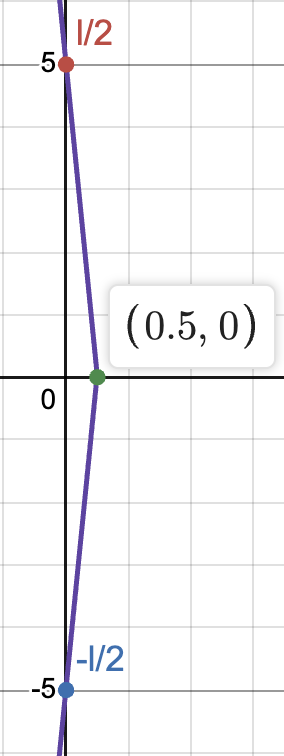
\includegraphics[width=0.2\textwidth]{./image/figure1.png}
                              \caption{Current Distribution of Small Dipole Antenna}
                        \end{figure}
            \end{enumerate}
      \item
            \[l = \frac{\lambda}{2} \text{, } f = 200 \times 10^6 \si{Hz}\text{, } \lambda = 1.5 \si{m} \text{, } R_{in} = R_{rad} = 73 \Omega \text{, }D_0 = 1.64 = 2.15 \si{dB}\]
            \begin{enumerate}[(i)]
                  \item $\boxed{l = 0.75}$.
                  \item $\boxed{G_0 = 2.51 \si{dB}}$.
                  \item We want $P_{rad} = 100 \si{W}$.

                        For a Half-wave Dipole Antenna,
                        \[\frac{1}{2}R_{in} |I_{in}|^2 = P_{rad}\]

                        Therefore,

                        \[|I_{in}| = \sqrt{\frac{2P_{rad}}{R_{in}}} = \boxed{1.66 \si{A}}\]
            \end{enumerate}
\end{enumerate}

\section{The reactance of small dipole antennas}
\begin{enumerate}[(a)]
      \item We know that the lumped element impedance of a transmission line, $Z_{in}$ with length $l$ is
            \[Z_{in} = z_0\left(\frac{z_L + j z_0 \tan(k l)}{z_0 + j z_L \tan(kl)}\right)\]

            Since $z_L = \infty$

            \[Z_{in} = z_0 \left(\frac{1}{j \tan(kl)}\right) = \boxed{-j \left(\frac{z_0}{\tan(kl)}\right)}\]
      \item $\boxed{\text{Capacitor}}$. The impedance resembles that of a capacitor $\left(\frac{-j}{\omega C}\right)$ at high frequency.
      \item The Short Dipole Antenna is like an open-end transmission line with $\frac{l}{\lambda} << 1$, which means $kl << 1$, so the short transmission line model in (a) shows that the antenna has a negative reactance and is equivalent to a capacitor.
      \item In the near field
            \[\widetilde{E}_{nf} = \frac{I_0 l k^2}{4\pi} \eta_0 \left(\frac{-j}{(kr)^3}\right)(2 \cos(\theta) \hat{r} + \sin(\theta) \hat{\theta})\]

            \[\widetilde{H}_{nf} = \frac{I_0 l k^2}{4\pi} \frac{1}{(kr)^2} \sin(\theta) \hat{\phi}\]

            \[\vec{S} = \widetilde{E}_{nf} \times \widetilde{H}_{nf} = \boxed{\left(\frac{I_0 l k^2}{4\pi}\right)^2 \eta_0 \left(\frac{-j}{(kr)^3}\right)\left(\frac{1}{(kr)^2}\right) (-2 \cos(\theta)\sin(\theta) \hat{\theta} + \sin^2(\theta) \hat{r})}\]
      \item
            \[\widetilde{V} = \widetilde{I}(-jX_C)\]
            \[S = \widetilde{I}\widetilde{V} = \boxed{(\widetilde{I})^2 (-jX_C)}\]
      \item Both complex power are similar because they are in the form of $(\text{current})^2 \times -j (\text{constant})$. This result suggests that the input impedance of the Short Dipole Antenna is purely reactive and negative.
      \item The time-average Poynting vector of the near field Hertzian Dipole Antenna is given by
            \[\vec{S}_{av} = \frac{1}{2}\text{Re}(\widetilde{E}_{nf} \times \widetilde{H}_{nf})\]

            However, we know that $\widetilde{E}_{nf} \times \widetilde{H}_{nf}$ is purely imaginary from (d). Therefore,
            \[\boxed{\vec{S}_{av} = 0}\]

            The result makes sense because we argued that the antenna behaves similarly to a capacitor in the near field. Capacitor's power is also purely imaginary because it only stores energy.
      \item $\boxed{\text{Inductor in series with the Small Dipole Antenna}}$. The Small Dipole Antenna is drawn as a capacitor in Figure 2.
            \begin{figure}[H]
                  \centering
                  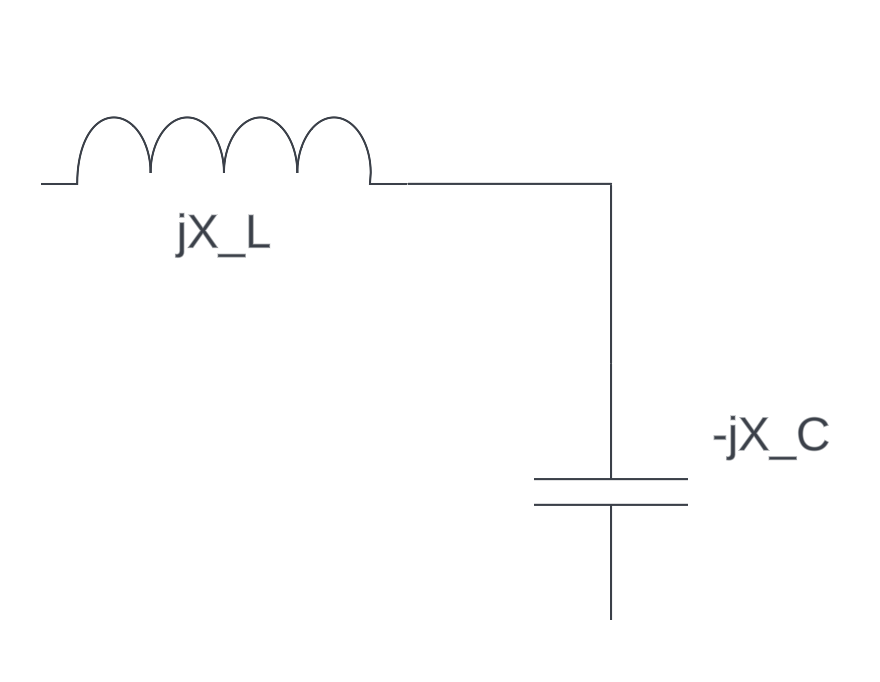
\includegraphics[width=0.4\textwidth]{./image/figure2.png}
                  \caption{Tune the Small Dipole Antenna}
            \end{figure}
\end{enumerate}

\section{Image charges and the quarter-wave monopole}
\subsection*{Image charges}
\addcontentsline{toc}{subsection}{Part 1: Image charges}
\begin{enumerate}[(a)]
      \item The right figure corresponds to an electric dipole, whose potential is
            \[V_{dipole} = \frac{qd \cos(\theta)}{2 \pi \epsilon r^2}\]
            Therefore, the electrostatic potential in this case is
            \[
                  V(r) =
                  \begin{cases}
                        \frac{qd \cos(\theta)}{2 \pi \epsilon r^2} & z \neq 0 \\
                        0                                          & z = 0    \\
                  \end{cases}
            \]
      \item \boxed{\text{Yes}}.
            \[\nabla^2 V(r) = \frac{1}{r^2} \frac{\partial}{\partial r} \left(r^2 \frac{\partial V(r)}{\partial r}\right) + \frac{1}{r^2 \sin(\theta)} \frac{\partial}{\partial \theta}\left(\sin(\theta)\frac{\partial V(r)}{\partial \theta}\right) = \frac{qd\cos(\theta)}{\pi \epsilon r^4} - \frac{qd\cos(\theta)}{\pi \epsilon r^4} = 0\]

            $V = 0$ when $z = 0$.

            The potential satisfies the boundary condition and the differential equation. Thus, it is a solution for the electrostatic potential.
      \item A dipole electric field will form between the charge and the surface because the configuration is equivalent to an electric dipole.
\end{enumerate}

\subsection*{Part 2: The quarter-wave monopole}
\addcontentsline{toc}{subsection}{Part 2: The quarter-wave monopole}
\begin{enumerate}[(a)]
      \item The left and right antenna are equivalent because the bottom part of right antenna have opposite polarity to that of the top antenna. Just like the image charge example from part 1, this configuration is equivalent to the left monopole antenna.
            The left monopole antenna has length $\frac{l}{2} = \frac{\lambda}{4}$, so a full antenna on the right is $2\frac{l}{2} = 2\frac{\lambda}{4} = \frac{\lambda}{2}$. Therefore, the monopole antenna is equivalent to a $\boxed{\text{Half Wave Dipole Antenna}}$.
      \item The voltage of the right antenna is twice of that or the left antenna despite both drives the same current. Therefore, the input impedance of the left monopole is half of that of the right antenna.
      \item A balun would not be needed because the monopole doesn't need to be driven by a differential signal like the Hertzian Dipole.
      \item Since $D_0 = 4\pi \left(\frac{U_{max}}{P_{rad}}\right)$, halving the total radiated power doubles the directivity of the dipole as $U_{max}$ is constant.

            Directivity of Half Wave Dipole = $1.64$.

            Therefore, $\boxed{D_0 = 3.28}$ for the monopole.
\end{enumerate}
\end{document}
